\chapter{Observations, matière noire et ajustement cosmologique}

\lectureoverview{Une observation ne prend sens que lorsqu’on la relie à un modèle cosmologique. Nous commençons par l’équation de Friedmann et les trois géométries spatiales homogènes, répartissons le contenu énergétique actuel de l’Univers entre rayonnement, matière, énergie du vide et courbure, puis reconstituons les raisons pour lesquelles un Univers ouvert a autrefois semblé inévitable. Les courbes de rotation des galaxies révèlent ensuite la matière gravitationnelle manquante et conduisent à la dynamique d’un halo froid, en faible interaction. Enfin, le décalage vers le rouge, la luminosité et le dénombrement des sources transforment une histoire d’expansion hypothétique en courbes observables. L’ancien modèle matière-courbure ne convient pas ; une fraction de matière proche de \(0.3\), une fraction d’énergie du vide proche de \(0.7\) et une courbure très faible donnent l’ajustement satisfaisant présenté dans ce cours.}

\section{Réintroduire les observations dans les équations}

Les faits astronomiques ne peuvent être interprétés isolément. Il faut d’abord disposer des équations qui indiquent quelles combinaisons d’observations permettent de distinguer les univers. Pour un univers homogène et isotrope, le point de départ est l’équation de Friedmann,
\begin{equation}
\left(\frac{\dot a}{a}\right)^2
=
\frac{8\pi G}{3}\rho-\frac{k}{a^2}.
\label{eq:c06-friedmann}
\end{equation}
La quantité
\begin{equation}
H(t)=\frac{\dot a(t)}{a(t)}
\label{eq:c06-hubble}
\end{equation}
est la \emph{fonction} de Hubble. Sa valeur actuelle \(H_0\) est conventionnellement appelée constante de Hubble, mais \(H(t)\) n’est pas constante au cours de l’histoire cosmique. Lorsque les astronomes donnent une valeur en kilomètres par seconde et par mégaparsec, ils donnent \(H_0\).

L’indice de courbure normalisé ne prend que trois valeurs,
\begin{equation}
k\in\{+1,0,-1\},
\end{equation}
qui correspondent respectivement aux géométries spatiales sphérique, plate et hyperbolique. La métrique FRW usuelle peut s’écrire
\begin{equation}
ds^2=-dt^2+a(t)^2\left[dr^2+\xi(r)^2d\Omega_2^2\right],
\label{eq:c06-frw}
\end{equation}
où
\begin{equation}
\xi(r)=
\begin{cases}
\sin r, & k=+1,\\
r, & k=0,\\
\sinh r, & k=-1.
\end{cases}
\label{eq:c06-xi}
\end{equation}
Cette notation remplit deux fonctions. Elle rassemble les trois géométries dans une même métrique et donne ensuite l’aire d’une sphère, donc le nombre de sources dans une coquille radiale. Le choix de \(k\) et une équation pour \(a(t)\) définissent ainsi déjà un modèle qui entraîne des conséquences observationnelles.

\section{Le contenu énergétique actuel de l’Univers}

Dans le modèle considéré, la densité d’énergie comporte trois composantes principales : le rayonnement, la matière non relativiste et l’énergie du vide. Si l’on ajoute la courbure au même bilan, on obtient
\begin{equation}
\frac{C_r}{a^4}
+\frac{C_m}{a^3}
+\Lambda
-\frac{k}{a^2}
=H^2.
\label{eq:c06-budget}
\end{equation}
Ici, \(\Lambda\) suit la normalisation du cours précédent, \(\Lambda=(8\pi G/3)\rho_{\rm vac}\). Le rayonnement se dilue comme \(a^{-4}\), la matière comme \(a^{-3}\), l’énergie du vide ne se dilue pas et la courbure évolue comme \(a^{-2}\). La courbure n’est pas une densité d’énergie matérielle, mais la placer à côté des autres termes rend la contrainte actuelle explicite : les quatre contributions doivent totaliser \(H_0^2\).

Définissons leurs fractions actuelles par
\begin{equation}
\begin{aligned}
\Omega_r&=\frac{C_r/a_0^4}{H_0^2},
&\qquad
\Omega_m&=\frac{C_m/a_0^3}{H_0^2},\\
\Omega_\Lambda&=\frac{\Lambda}{H_0^2},
&
\Omega_k&=\frac{-k/a_0^2}{H_0^2}.
\end{aligned}
\label{eq:c06-omegas}
\end{equation}
On a alors
\begin{equation}
\boxed{\Omega_r+\Omega_m+\Omega_\Lambda+\Omega_k=1.}
\label{eq:c06-sum-rule}
\end{equation}
Les \(\Omega\) sont des rapports évalués aujourd’hui, et non des constantes indépendantes du temps. Notons également la convention de signe : \(k=-1\) donne une valeur positive de \(\Omega_k\).

\subsection{Comment mesurer les premiers termes}

Hubble a obtenu le taux d’expansion local en comparant le décalage vers le rouge dû à la récession à la distance. À faible \(z\), le décalage vers le rouge fournit une vitesse ; une luminosité étalonnée donne une distance. Sa première valeur numérique était très erronée, mais la méthode était juste. Les galaxies étant relativement proches, la mesure ne sondait qu’une faible fraction de l’histoire cosmique et l’on pouvait prendre \(H\) pour sa valeur actuelle.

\begin{classroomqa}
\audiencequestion{Comment la luminosité peut-elle donner la distance si la luminosité intrinsèque n’est pas déjà connue ?}
\lecturerresponse{Cela ne peut se faire en une seule étape. L’échelle des distances cosmiques commence par la parallaxe des étoiles proches. Les étoiles variables céphéides de cette région étalonnée révèlent une relation période-luminosité et deviennent des chandelles standard pour mesurer de plus grandes distances. Des étalonnages qui se recouvrent prolongent l’échelle, et les supernovæ fournissent les meilleures chandelles aux décalages cosmologiques utilisés plus loin. La distance est donc déduite d’une chaîne d’étalons, et non d’une hypothèse arbitraire selon laquelle tous les objets brilleraient de la même façon. \lecturetimestamp{00:10:00--00:11:32}}
\end{classroomqa}

\begin{classroomqa}
\audiencequestion{\(C_r\) et \(C_m\) sont-ils des constantes alors que leurs densités varient ?}
\lecturerresponse{Oui. Les coefficients restent fixes, tandis que les facteurs \(a^{-4}\) et \(a^{-3}\) portent la dépendance temporelle. L’énergie du vide est constante et la courbure évolue comme \(a^{-2}\). C’est précisément en raison de ces puissances différentes que les contributions relatives varient d’une époque à l’autre. \lecturetimestamp{00:11:35--00:12:02}}
\end{classroomqa}

Le terme de rayonnement peut être mesuré localement à partir du fond photonique. Il s’agit principalement du fond diffus cosmologique, dont la densité d’énergie actuelle est infime devant celle des autres composantes importantes. Il faut considérer un volume de moyennage suffisamment grand, mais nul besoin de remonter loin le cône de lumière passé pour établir que \(\Omega_r\) est négligeable aujourd’hui.

La matière visible est estimée à partir des galaxies, des populations stellaires, de l’hydrogène et du gaz interstellaire. Les méthodes sont techniques, mais les idées ne sont pas obscures : déterminer le contenu typique en étoiles et en gaz, le sommer sur l’ensemble des galaxies, puis calculer la moyenne dans un grand volume. Le cours cite l’ordre de grandeur approximatif ancien d’une masse de proton par mètre cube. C’est beaucoup plus que la densité de rayonnement, mais cela reste remarquablement ténu.

\begin{classroomqa}
\audiencequestion{Qu’en est-il de la matière noire dans ce bilan ?}
\lecturerresponse{Nous y arrivons, mais commençons délibérément par reconstituer l’ancienne inférence fondée uniquement sur la matière lumineuse. L’ordre historique importe : il montre précisément quelle conclusion apparente la matière noire a corrigée et quelle lacune elle n’a pas comblée. \lecturetimestamp{00:15:08--00:15:40}}
\end{classroomqa}

\section{Pourquoi un Univers ouvert a autrefois semblé nécessaire}

Dans l’ancien tableau, on jugeait à juste titre le rayonnement négligeable, on posait l’énergie du vide égale à zéro et l’on entendait par matière uniquement celle qui est visible par son rayonnement électromagnétique. L’estimation qui en résultait était approximativement
\begin{equation}
\Omega_r\simeq0,
\qquad
\Omega_\Lambda=0,
\qquad
\Omega_m^{\rm luminous}\sim\frac{1}{20}\text{--}\frac{1}{30}.
\end{equation}
La règle de somme semblait alors imposer
\begin{equation}
\Omega_k\simeq1.
\end{equation}
Comme une contribution positive du terme de courbure signifie \(-k/a_0^2>0\), on en déduisait \(k=-1\) : un Univers ouvert à courbure négative. Ces nombres reconstituent l’ancien raisonnement ; ils ne constituent pas une estimation moderne des paramètres.

Pour interpréter l’échelle de courbure, revenons à la solution dominée par la matière
\begin{equation}
a(t)\propto t^{2/3}.
\end{equation}
En dérivant et en divisant par \(a\), on obtient
\begin{equation}
H(t)=\frac{\dot a}{a}=\frac{2}{3t}.
\label{eq:c06-matter-h}
\end{equation}
À l’âge actuel \(T\),
\begin{equation}
H_0\simeq\frac{2}{3T}.
\end{equation}
Le temps de Hubble est donc du même ordre que l’âge de l’Univers. La comparaison avec l’ère dominée par le rayonnement,
\begin{equation}
a(t)\propto t^{1/2},
\qquad
H(t)=\frac{1}{2t},
\end{equation}
montre que cette relation entre l’inverse de l’âge et le taux d’expansion ne caractérise pas uniquement la poussière.

\begin{figure}[htbp]
\centering
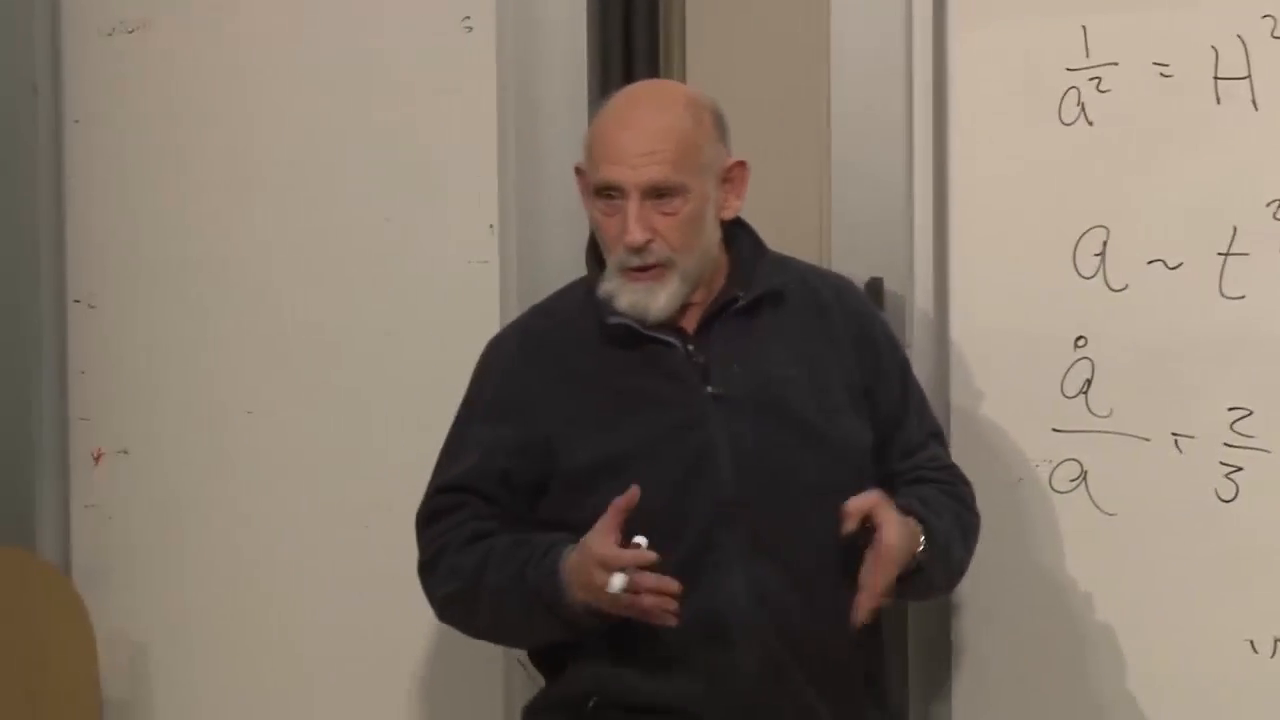
\includegraphics[width=0.72\textwidth]{lecture_06_figure_02.png}
\caption{Récapitulatif au tableau pour l’ère dominée par la matière. On distingue les expressions \(a\sim t^{2/3}\) et \(\dot a/a=2/(3t)\) ; le chargé de cours masque le reste du tableau, de sorte qu’aucune équation cachée n’est attribuée à l’image.}
\label{fig:c06-age-board}
\lectureframe{00:24:41.615}
\end{figure}

\begin{classroomqa}
\audiencequestion{Quelles sont les unités de la constante de Hubble, et où intervient la vitesse de la lumière ?}
\lecturerresponse{Puisque \(H\) relie une vitesse à une distance, cette quantité a l’unité de l’inverse d’un temps. On peut l’exprimer en secondes inverses, en années inverses ou, de manière équivalente, dans l’unité astronomique de kilomètres par seconde et par mégaparsec. La relation \(H\sim1/T\) ne nécessite aucun facteur supplémentaire de \(c\). Un facteur \(c\) n’apparaît que lorsque le temps \(T\) est converti en une longueur telle que \(cT\). \lecturetimestamp{00:22:50--00:24:25}}
\end{classroomqa}

La valeur initiale de \(H_0\) donnée par Hubble était trop grande d’environ un ordre de grandeur ; l’âge de Hubble correspondant était donc trop court : de l’ordre du milliard plutôt que de dix milliards d’années dans la comparaison arrondie du cours. Un meilleur étalonnage a corrigé la valeur sans remettre en cause l’idée que \(H_0^{-1}\) est une échelle de temps cosmique.

L’ancienne inférence sur la courbure s’écrit maintenant
\begin{equation}
\frac{1}{a_0^2}\sim H_0^2\sim\frac{1}{T^2}.
\end{equation}
Dans les unités où \(c=1\), on pensait donc que le rayon de courbure \(a_0\) était de l’ordre de l’âge \(T\) ; en rétablissant les unités usuelles, il était de l’ordre de \(cT\). Le cours précise aussitôt que cette affirmation ne décrit pas l’Univers réel. C’était la conclusion à laquelle on arrivait plusieurs décennies auparavant, après avoir écarté les termes alors jugés négligeables.

\begin{classroomqa}
\audiencequestion{Si la courbure était censée dominer aujourd’hui, pourquoi utiliser la loi de domination de la matière \(a\propto t^{2/3}\) ?}
\lecturerresponse{Parce que la matière évolue comme \(a^{-3}\), tandis que la courbure ne varie que comme \(a^{-2}\). Lorsque \(a\) est plus petit, la matière l’emporte. La courbure ne pouvait devenir importante que tardivement ; la domination de la matière décrivait donc toujours la majeure partie de l’histoire écoulée et maintenait \(H_0\) à un ordre de grandeur de \(1/T\). Une solution complète mêlant les deux composantes corrigerait le facteur numérique, sans effacer l’argument d’échelle de temps. \lecturetimestamp{00:49:20--00:50:17}}
\end{classroomqa}

\section{La matière noire révélée par la dynamique galactique}

Il existe deux façons opérationnelles de recenser la matière. La première consiste à compter ce qui émet ou absorbe de la lumière ; la seconde, à déduire la masse de la gravité. Au début des années 1930, Oort a découvert une anomalie dans la dynamique galactique, et Zwicky a constaté un écart de masse analogue dans les amas de galaxies. Les observations indiquaient que la matière gravitationnelle dépassait la matière lumineuse. La matière ordinaire, chargée, rayonne et entre en collision ; la composante manquante a d’abord été identifiée par son action gravitationnelle.

\begin{classroomqa}
\audiencequestion{La matière lumineuse comprend-elle le gaz diffus et les trous noirs centraux ?}
\lecturerresponse{Le gaz diffus est inclus dans la mesure où l’on peut en déduire la quantité à partir de son comportement électromagnétique. Un trou noir supermassif central peut être inclus dans le bilan de masse connu, mais il ne représente qu’une petite fraction de la masse totale de la galaxie et reste concentré au centre. Il ne peut expliquer un écart qui persiste bien au-delà du centre lumineux. \lecturetimestamp{00:29:50--00:31:14}}
\end{classroomqa}

Considérons une étoile qui se déplace approximativement sur une orbite circulaire de rayon \(r\). Si presque toute la masse \(M\) était concentrée près du centre galactique, la loi de Newton donnerait
\begin{equation}
\frac{GM}{r^2}=\frac{v^2}{r},
\end{equation}
et donc
\begin{equation}
v^2=\frac{GM}{r},
\qquad
v(r)\propto r^{-1/2}.
\label{eq:c06-kepler}
\end{equation}
C’est la décroissance képlérienne attendue à l’extérieur d’une distribution de masse centrale.

\begin{figure}[htbp]
\centering
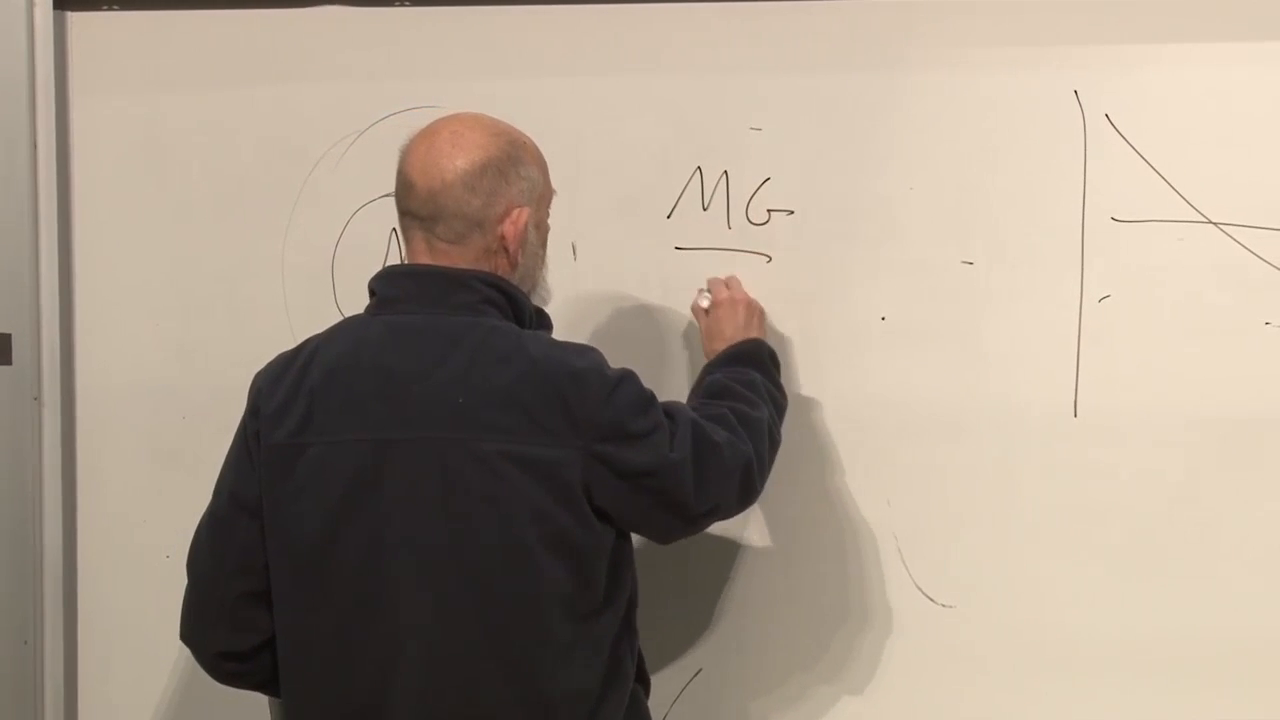
\includegraphics[width=0.78\textwidth]{lecture_06_figure_03.png}
\caption{Tableau des courbes de rotation, où l’on passe d’une masse centrale à la masse intérieure \(M(r)\). Seuls \(MG\), la barre de fraction, le schéma de l’orbite et des parties des croquis de courbe sont visibles ; l’équation ~\eqref{eq:c06-kepler} provient du raisonnement oral.}
\label{fig:c06-rotation-board}
\lectureframe{00:34:53.642}
\end{figure}

\begin{figure}[htbp]
\centering
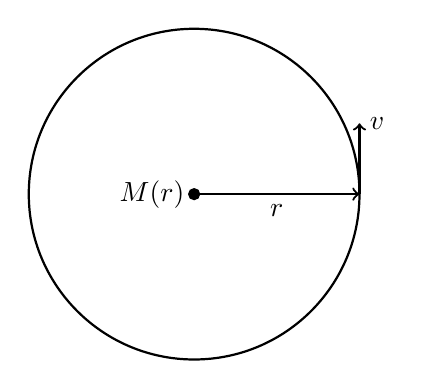
\begin{tikzpicture}[scale=1.0]
\filldraw (0,0) circle (2pt) node[left] {\(M(r)\)};
\draw[thick] (0,0) circle (2.1);
\draw[->,thick] (0,0)--(2.1,0) node[midway,below] {\(r\)};
\draw[->,thick] (2.1,0)--(2.1,0.9) node[right] {\(v\)};
\end{tikzpicture}
\caption{Construction de l’orbite circulaire utilisée pour déduire la masse intérieure à partir de la vitesse de rotation mesurée.}
\label{fig:c06-orbit-redraw}
\end{figure}

Les courbes de rotation galactiques observées ne décroissent pas ainsi ; elles sont approximativement plates sur une plage radiale importante. Remplaçons la masse centrale fixe par la masse intérieure \(M(r)\) :
\begin{equation}
\frac{G M(r)}{r^2}=\frac{v(r)^2}{r}.
\end{equation}
Si \(v(r)\) est presque constante, alors
\begin{equation}
\boxed{M(r)\propto r.}
\label{eq:c06-enclosed-mass}
\end{equation}
Il s’agit de la masse totale à l’intérieur du rayon \(r\), et non de la densité locale. La masse gravitationnelle continue d’augmenter bien au-delà de la région où se concentre l’essentiel de la lumière des étoiles. Les mouvements perpendiculaires aux disques galactiques indiquent en outre une distribution approximativement sphérique : un halo sombre plutôt qu’un second disque mince.

\begin{classroomqa}
\audiencequestion{Existe-t-il une théorie simple qui explique pourquoi la courbe de rotation est si plate ?}
\lecturerresponse{Pas dans le cadre de ce raisonnement. Les simulations de formation des galaxies peuvent rendre ces profils naturels, mais le cours ne prétend pas en donner une dérivation courte. Le résultat solidement établi est observationnel : une valeur de \(v\) presque constante implique que la masse intérieure croît approximativement de façon linéaire. L’élégance de cette relation ne doit pas être confondue avec une explication élémentaire de la formation des galaxies. \lecturetimestamp{00:35:58--00:37:33}}
\end{classroomqa}

\begin{classroomqa}
\audiencequestion{Les bras spiraux sont-ils simplement des moulinets matériels engendrés par la variation de la vitesse angulaire \(v/r\) ?}
\lecturerresponse{Aucune image simple de moulinet ne convient. Le motif visible n’est pas nécessairement solidaire de la rotation des étoiles individuelles ; les descriptions en termes d’ondes de densité ou d’ondes de formation stellaire font partie des possibilités. Le cours s’appuie sur cette incertitude pour distinguer l’inférence robuste concernant le halo du problème plus complexe de la structure spirale. \lecturetimestamp{00:37:35--00:38:34; 00:47:03--00:47:47}}
\end{classroomqa}

La masse noire déduite est plusieurs fois supérieure à la masse lumineuse ; le cours la situe seulement dans un ordre de grandeur compris entre environ cinq et dix. Le halo s’étend également au-delà de la galaxie visible. Ces échelles sont volontairement approximatives et historiques ; elles ne sont pas des rapports universels précis valables pour chaque système.

\section{Les propriétés requises de la matière noire}

Pourquoi la matière ordinaire forme-t-elle des disques lumineux et compacts, alors que la matière noire reste répartie dans un large halo ? La matière lumineuse peut perdre de l’énergie mécanique par collisions électromagnétiques et par rayonnement. En dissipant son énergie, elle peut être attirée par la gravité vers une configuration plus dense. La matière noire semble électriquement neutre et interagir beaucoup plus faiblement. Ses particules parcourent le halo avec peu de collisions ou de rayonnement ; même en plusieurs milliards d’années, elles ne perdent donc pas assez d’énergie pour s’installer dans le disque lumineux. Le rayonnement gravitationnel dû au mouvement galactique est beaucoup trop faible pour constituer un mécanisme de refroidissement de remplacement.

\begin{classroomqa}
\audiencequestion{Dire que la matière noire interagit faiblement signifie-t-il qu’elle obéit à une autre loi de la gravité ?}
\lecturerresponse{Non. On suppose qu’elle subit la gravitation de la manière habituelle. Ici, « interaction faible » signifie que les collisions autres que gravitationnelles et le rayonnement électromagnétique sont absents ou fortement supprimés. Deux particules noires s’attirent toujours gravitationnellement ; cette attraction organise un halo, mais ne dissipe pas efficacement l’énergie orbitale. \lecturetimestamp{00:42:36--00:43:35}}
\end{classroomqa}

\begin{classroomqa}
\audiencequestion{Quelles observations montrent qu’il ne s’agit pas seulement d’une particularité d’une courbe de rotation galactique ?}
\lecturerresponse{Les indices apparaissent à plusieurs échelles : mouvements des étoiles dans les galaxies, mouvements perpendiculaires aux plans galactiques, interactions entre galaxies et dynamique des amas entiers de galaxies. Les exemples d’Oort et de Zwicky étaient des manifestations différentes du même problème de gravité manquante. \lecturetimestamp{00:42:00--00:42:36}}
\end{classroomqa}

\begin{classroomqa}
\audiencequestion{La matière noire devrait-elle se concentrer autour des trous noirs et des centres galactiques ?}
\lecturerresponse{Sa densité augmente bien en direction d’un centre gravitationnel, mais la séquence historique s’est probablement déroulée à l’inverse d’un halo formé autour d’un trou noir préexistant. Les halos noirs ont créé de grands puits gravitationnels ; la matière baryonique y est ensuite tombée et a formé les galaxies, les étoiles et les trous noirs centraux. Le trou noir ne représente qu’une petite part de la masse. Les recherches de produits d’annihilation se tournent néanmoins vers le centre galactique, où la densité de matière noire devrait être plus élevée. \lecturetimestamp{00:43:36--00:45:43}}
\end{classroomqa}

\begin{classroomqa}
\audiencequestion{La matière noire est-elle un gaz, de la poussière, des amas compacts ou des particules isolées ? Une partie pourrait-elle être piégée près du Soleil ?}
\lecturerresponse{Sa nature microscopique est inconnue, mais la poussière ordinaire est liée par des forces électromagnétiques, précisément le type d’interactions qui semble manquer à la matière noire. L’image usuelle est donc celle d’une population clairsemée de particules individuelles. Certaines pourraient être concentrées gravitationnellement près du Soleil, mais leur densité est bien trop faible pour rivaliser avec la gravité solaire ou perturber la dynamique planétaire. \lecturetimestamp{00:45:43--00:47:02; 00:58:41--00:59:29}}
\end{classroomqa}

La deuxième condition essentielle est que la matière noire puisse s’agréger. Une population chaude, dont les vitesses aléatoires sont relativistes, résiste à l’agrégation gravitationnelle ; une population froide peut tomber dans les puits de potentiel. Les neutrinos ordinaires légers auraient constitué une matière noire chaude et ne peuvent fournir la composante galactique principale requise. Dans ce contexte, \emph{froide} signifie non relativiste dans le référentiel cosmologique local, et non à une température littéralement nulle en laboratoire.

\begin{classroomqa}
\audiencequestion{La condition d’une agrégation à froid impose-t-elle une plage de masses pour la matière noire ?}
\lecturerresponse{Cela dépend des statistiques quantiques et de l’histoire de production. Les fermions très légers ne peuvent pas tous occuper un même état lent et sont fortement contraints. Les bosons très légers peuvent occuper un état cohérent de condensation de Bose-Einstein ; les axions en sont l’exemple donné dans le cours. Autre possibilité : des particules plus lourdes, en faible interaction, peuvent être froides sans condensation. Cet argument ne fournit donc pas de limite de masse unique indépendante du modèle. \lecturetimestamp{00:53:17--00:54:52; 00:56:42--00:58:05}}
\end{classroomqa}

\begin{classroomqa}
\audiencequestion{Les accélérateurs auraient-ils déjà dû découvrir ces particules ?}
\lecturerresponse{Seulement sous des hypothèses supplémentaires. Si les particules ont des sections efficaces d’interaction de l’ordre de celles de l’interaction faible et des masses accessibles aux accélérateurs, leur production en collisionneur est peut-être possible. L’espoir, exprimé dans le cours, d’obtenir prochainement des informations était explicitement spéculatif et lié à l’époque. Une particule pourrait au contraire être trop lourde ou interagir trop faiblement pour les expériences disponibles. \lecturetimestamp{00:54:52--00:55:54}}
\end{classroomqa}

\begin{classroomqa}
\audiencequestion{La matière noire pourrait-elle simplement se trouver dans une dimension supplémentaire invisible ?}
\lecturerresponse{Aucun mécanisme de ce type n’est nécessaire dans cette discussion. La matière noire est déjà observée par ses effets gravitationnels et pourrait simplement être constituée de particules inhabituelles, presque dépourvues d’interaction avec la matière ordinaire. Dire qu’une interaction est faible ne revient pas à placer les particules en dehors de l’espace-temps observable. \lecturetimestamp{00:55:54--00:56:41}}
\end{classroomqa}

Modifier la gravité au lieu d’ajouter de la matière invisible est une alternative logique. Selon le cours, aucune modification aussi simple n’expliquait alors les observations à toutes les échelles pertinentes tout en préservant les lois qui fonctionnent dans le Système solaire. L’interprétation en termes de particules est donc privilégiée, mais leur microphysique reste inconnue.

\section{La matière noire ne ferme pas l’ancien bilan}

La matière noire augmente de plusieurs fois la contribution de la matière, mais l’ancien écart entre la matière lumineuse et \(H_0^2\) était de l’ordre de vingt-cinq. Elle réduit donc l’écart sans permettre d’obtenir
\begin{equation}
\frac{C_m}{a_0^3}=H_0^2.
\end{equation}
Dans le cadre ancien où \(\Lambda\) était exclue, un terme positif dans le bilan de courbure, et donc \(k<0\), restait nécessaire. Ce modèle ouvert n’avait rien d’incohérent sur le plan logique ; l’idée est que la matière noire, à elle seule, ne permettait pas de retrouver la réponse moderne.

\begin{classroomqa}
\audiencequestion{Que pensaient réellement les cosmologistes de la courbure avant l’ajustement moderne ?}
\lecturerresponse{Les observations prêtaient à confusion, et la préférence préalable pour un Univers fermé et borné allait parfois à l’encontre du bilan de matière. Une fois les anciennes hypothèses combinées de façon cohérente, la courbure négative s’imposait naturellement. Ce consensus historique restait provisoire, car ni la matière noire ni l’énergie du vide n’étaient intégrées de manière aussi solide qu’aujourd’hui. \lecturetimestamp{00:50:17--00:51:50}}
\end{classroomqa}

Il faut donc tester le modèle candidat au lieu d’en déduire la validité d’une seule ligne de bilan. Un modèle consiste en un choix de courbure \(k\) et une histoire d’expansion \(a(t)\), ou, de façon équivalente, en un ensemble d’équations d’état pour la matière et de paramètres actuels à partir desquels on calcule \(a(t)\). L’ancien modèle candidat associe matière et courbure négative, avec un rayonnement négligeable et sans constante cosmologique.

\section{De la géométrie aux observables}

\subsection{Dénombrement et luminosité des sources dans une géométrie figée}

Mettons provisoirement de côté l’évolution cosmique. Dans un univers homogène, le nombre de sources dans une coquille comobile est proportionnel à son aire :
\begin{equation}
dN\propto \xi(r)^2\,dr.
\label{eq:c06-shell-count}
\end{equation}
On a donc
\begin{equation}
dN\propto
\begin{cases}
\sin^2r\,dr, & k=+1,\\
r^2\,dr, & k=0,\\
\sinh^2r\,dr, & k=-1.
\end{cases}
\end{equation}
Aux grandes valeurs de \(r\), le cas à courbure négative croît comme \(\sinh^2r\sim e^{2r}\), bien plus rapidement que la loi plate \(r^2\). La courbure négative prédit donc une augmentation anormalement rapide du nombre de sources avec la distance.

La même aire détermine le flux reçu. Dans un espace plat et statique, une source standard donne
\begin{equation}
F\propto\frac{1}{r^2}.
\end{equation}
Dans un espace hyperbolique, la sphère sur laquelle se répartit le rayonnement croît plus vite ; le flux diminue donc plus rapidement. Le cours appelle parfois cette quantité observée « luminosité » ; ici, \(F\) désigne l’éclat ou le flux, tandis que la luminosité intrinsèque est une propriété de la source. Le dénombrement et la luminosité permettent donc, ensemble, de distinguer les géométries spatiales.

\subsection{Décalage vers le rouge et cône de lumière passé}

L’Univers réel évolue, et regarder au loin revient à regarder dans le passé. La lumière émise à \(t_{\rm em}\) est étirée tandis que le facteur d’échelle passe de \(a(t_{\rm em})\) à \(a_0\) :
\begin{equation}
1+z
=\frac{\lambda_{\rm obs}}{\lambda_{\rm em}}
=\frac{a_0}{a(t_{\rm em})}.
\label{eq:c06-redshift}
\end{equation}
De manière équivalente,
\begin{equation}
z=\frac{\lambda_{\rm obs}}{\lambda_{\rm em}}-1.
\end{equation}
Différents points de notre cône de lumière passé correspondent simultanément à des rayons comobiles différents et à des instants d’émission différents. L’expansion modifie la longueur d’onde ; le décalage Doppler et le décalage gravitationnel sont d’autres mécanismes physiques, mais c’est l’effet de l’expansion cosmologique qui nous intéresse ici.

\begin{classroomqa}
\audiencequestion{Pourquoi la définition de \(z\) comporte-t-elle un terme moins un ?}
\lecturerresponse{C’est une convention historique, choisie pour qu’une source sans décalage ait \(z=0\). Le facteur d’étirement directement physique est \(1+z=\lambda_{\rm obs}/\lambda_{\rm em}\). \lecturetimestamp{01:10:11--01:10:45}}
\end{classroomqa}

Pour un rayon radial, \(d\Omega_2=0\) et \(ds^2=0\). L’équation ~\eqref{eq:c06-frw} donne donc
\begin{equation}
dt^2=a(t)^2dr^2.
\end{equation}
Pour un rayon entrant, que l’on suit à rebours à partir de notre position,
\begin{equation}
dt=-a(t)\,dr,
\qquad
\frac{dr}{dt}=-\frac{1}{a(t)}.
\label{eq:c06-null-ray}
\end{equation}
Le signe moins indique que les grands rayons comobiles correspondent aux temps plus anciens le long du rayon. Une fois \(a(t)\) connue, cette équation détermine \(r(t)\).

\subsection{Nombre par intervalle de décalage vers le rouge}

Un observateur peut compter les sources standard dans un intervalle de décalage vers le rouge allant de \(z\) à \(z+dz\). Partons de l’équation ~\eqref{eq:c06-shell-count} et dérivons l’équation ~\eqref{eq:c06-redshift} le long du rayon lumineux passé :
\begin{equation}
dz=-\frac{a_0}{a^2}\,da
=-\frac{a_0}{a^2}\dot a\,dt.
\end{equation}
En utilisant \(dt=-a\,dr\),
\begin{equation}
dz=\frac{a_0}{a}\dot a\,dr
=(1+z)\dot a\,dr.
\end{equation}
On obtient donc
\begin{equation}
dr=\frac{dz}{(1+z)\dot a},
\end{equation}
et, pour une densité comobile de sources fixée,
\begin{equation}
\boxed{
\frac{dN}{dz}
\propto
\frac{\xi(r)^2}{(1+z)\dot a}
}.
\label{eq:c06-dndz}
\end{equation}
Le calcul au tableau vérifie plusieurs fois les signes et les facteurs ; les équations ~\eqref{eq:c06-null-ray} et \eqref{eq:c06-redshift} fixent sans ambiguïté le résultat.

\begin{figure}[htbp]
\centering
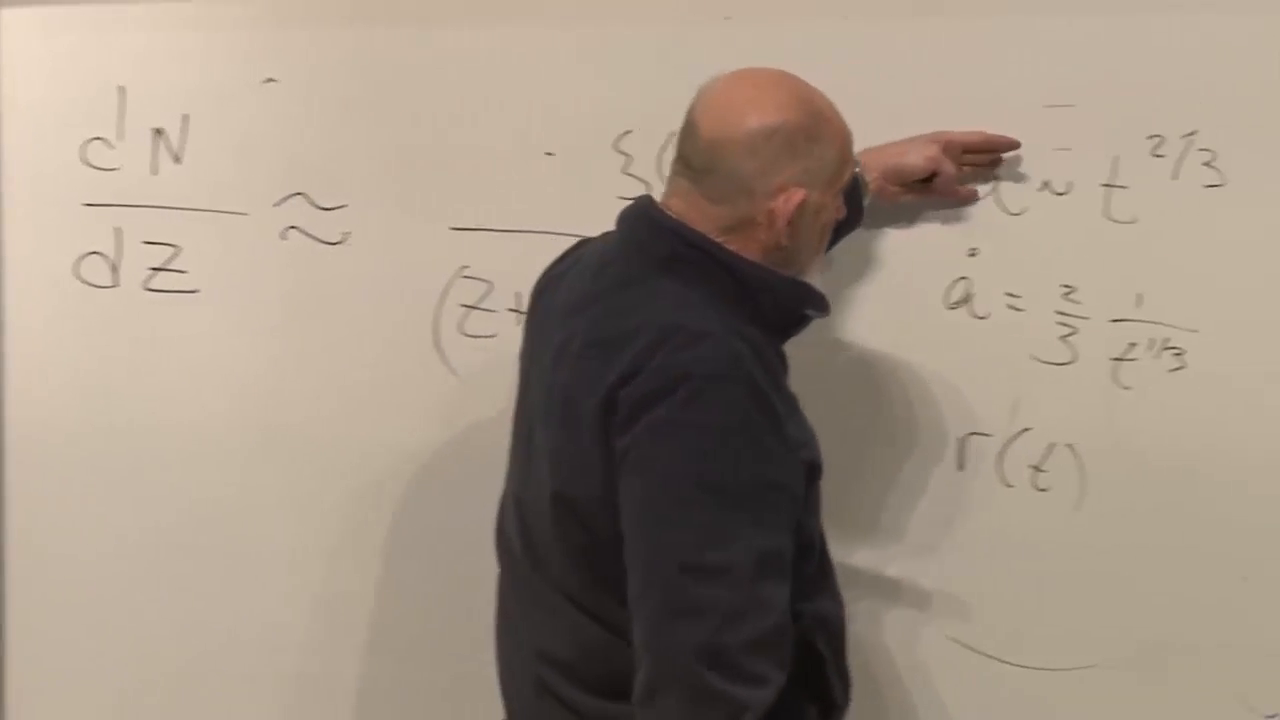
\includegraphics[width=0.84\textwidth]{lecture_06_figure_05.png}
\caption{Relation au tableau entre \(dN/dz\) et les fonctions du modèle. Le membre de gauche, ainsi que \(a\sim t^{2/3}\), \(\dot a\) et \(r(t)\) à droite, sont visibles, mais le chargé de cours masque une partie du dénominateur ; l’équation ~\eqref{eq:c06-dndz} a été établie indépendamment plus haut.}
\label{fig:c06-dndz-board}
\lectureframe{01:22:24.114}
\end{figure}

Il n’y a rien d’autre à calculer avant d’avoir choisi un modèle. Une fonction \(a(t)\) spécifiée détermine \(\dot a(t)\), l’équation ~\eqref{eq:c06-null-ray} détermine \(r(t)\) et l’équation ~\eqref{eq:c06-redshift} permet d’exprimer chaque quantité en fonction de \(z\). Des équations d’état différentes produisent des fonctions \(dN/dz\) et \(F(z)\) différentes. C’est précisément ce qui rend les observations discriminantes.

\section{Des paramètres d’essai au meilleur ajustement}

La procédure est directe :
\begin{equation}
(\Omega_r,\Omega_m,\Omega_\Lambda,\Omega_k)
\longrightarrow
a(t)
\longrightarrow
\left\{F(z),\frac{dN}{dz}\right\}.
\label{eq:c06-fit-pipeline}
\end{equation}
Choisir les paramètres actuels, résoudre l’équation de Friedmann, propager la lumière radiale, calculer la luminosité et le dénombrement en fonction du décalage vers le rouge, puis comparer les courbes aux données. Une comparaison infructueuse conduit à rejeter le jeu de paramètres. Ensemble, les deux observables contraignent à la fois l’histoire de l’expansion et la géométrie spatiale.

\begin{figure}[htbp]
\centering
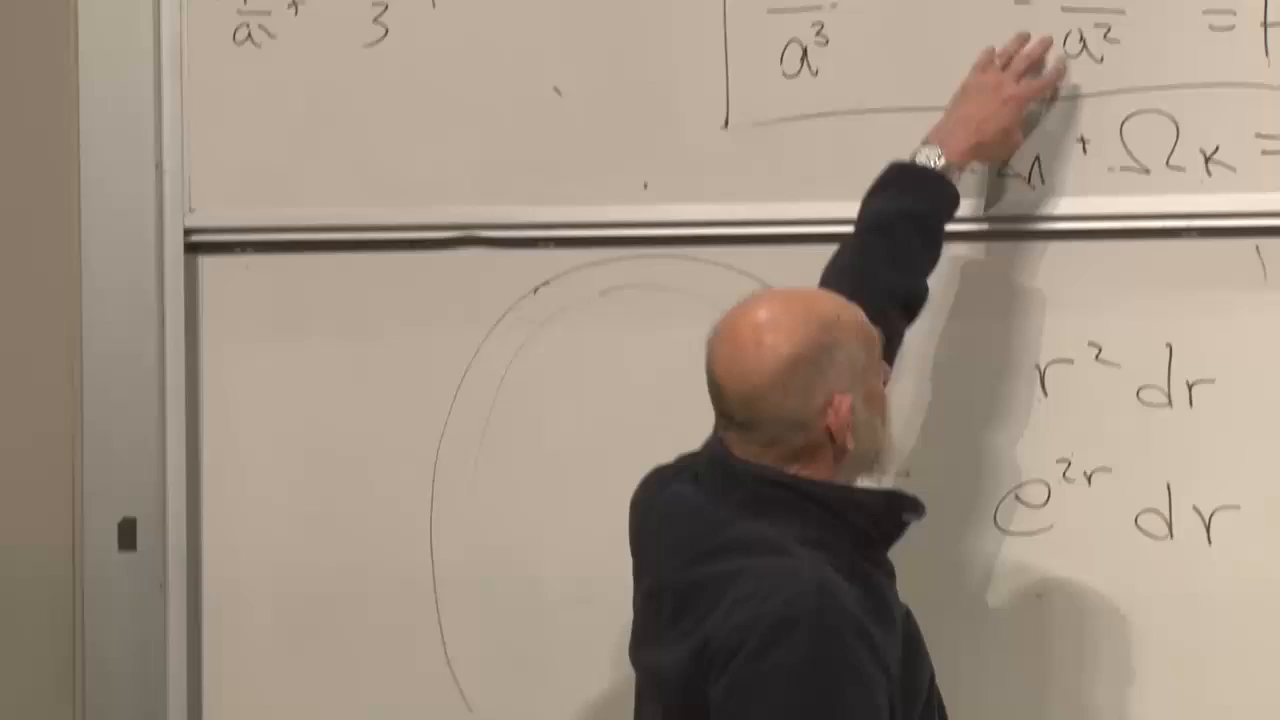
\includegraphics[width=0.84\textwidth]{lecture_06_figure_06.png}
\caption{Ancien modèle matière-courbure au tableau du haut, et facteurs de coquille plate et hyperbolique \(r^2dr\) et \(e^{2r}dr\) au tableau du bas. Des parties de l’équation de Friedmann sont masquées ; cette image apporte donc un élément d’appui, mais ne constitue pas une source d’équation.}
\label{fig:c06-old-model-board}
\lectureframe{01:24:27.863}
\end{figure}

L’ancien modèle,
\begin{equation}
H^2=\frac{C_m}{a^3}-\frac{k}{a^2},
\qquad k=-1,
\end{equation}
ne reproduit ni la relation entre luminosité et décalage vers le rouge, ni le test du dénombrement des sources. Les supernovæ fournissent les chandelles standard les plus utiles dans l’intervalle de décalage vers le rouge pertinent. Le jeu de paramètres qui donne l’ajustement satisfaisant dans le cours est
\begin{equation}
\boxed{
\Omega_r\simeq0,\qquad
\Omega_m\simeq0.3,\qquad
\Omega_\Lambda\simeq0.7,\qquad
\Omega_k\simeq0
}.
\label{eq:c06-best-fit}
\end{equation}
Ici, la matière inclut la matière lumineuse et la matière noire. Ces valeurs correspondent à l’ajustement présenté à l’époque du cours ; la leçon durable porte sur la méthode d’ajustement et la nécessité d’une composante dominante qui ne se dilue pas, et non sur la dernière décimale imprimée.

\subsection{Questions sur les mesures et les paramètres ajustés}

\begin{classroomqa}
\audiencequestion{\(\Lambda\) était-elle déjà supposée dans la discussion de l’ancien modèle d’Univers ouvert ?}
\lecturerresponse{Non. La première partie reconstituait délibérément l’ancien modèle en posant \(\Lambda=0\). Les valeurs de l’équation ~\eqref{eq:c06-best-fit} décrivent l’ajustement moderne, établi plus tard. L’ancien modèle candidat n’a pas été modifié subrepticement : il a été confronté à \(F(z)\) et à \(dN/dz\), et n’a pas résisté à ces tests. \lecturetimestamp{01:26:45--01:27:07}}
\end{classroomqa}

\begin{classroomqa}
\audiencequestion{Comment obtient-on \(\Omega_\Lambda\) si l’énergie du vide n’est pas mesurée directement comme la matière locale ?}
\lecturerresponse{On commence par essayer différents jeux de paramètres. Chacun définit une solution de Friedmann et, par conséquent, les fonctions prédites \(F(z)\) et \(dN/dz\). On compare ces prédictions aux observations, on écarte les mauvais ajustements et on retient la meilleure région de l’espace des paramètres. La valeur \(0.7\) est déduite de l’ajustement ; elle ne provient pas d’une lecture directe sur un appareil de mesure de l’énergie du vide. \lecturetimestamp{01:27:08--01:29:59; 01:31:57--01:33:40}}
\end{classroomqa}

\begin{classroomqa}
\audiencequestion{D’où vient l’échelle actuelle \(a_0\) ?}
\lecturerresponse{La normalisation de \(a\) est en partie conventionnelle, mais un modèle achevé, fixé par \(H_0\), fournit l’échelle physique actuelle de courbure lorsque \(k\ne0\). Une fois que le modèle reproduit les observables liées au décalage vers le rouge, sa fonction \(a(t)\) repère le point actuel et l’échelle correspondante. \lecturetimestamp{01:29:59--01:30:42}}
\end{classroomqa}

\begin{classroomqa}
\audiencequestion{Le fait de regarder des milliards d’années dans le passé fausse-t-il un ajustement fondé sur les paramètres actuels ?}
\lecturerresponse{Regarder dans le passé ne fausse pas l’ajustement : c’est précisément le signal. On insère les paramètres actuels dans l’équation de Friedmann, qui les fait évoluer pour donner un \(a(t)\) complet. Le cône de lumière prédit tient déjà compte du fait que la matière avait davantage d’importance lorsque \(a\) était plus petit, et que le rayonnement finit par dominer suffisamment loin dans le passé. Un modèle qui négligerait cette évolution ne rendrait pas compte des données. \lecturetimestamp{01:30:43--01:31:55}}
\end{classroomqa}

\begin{classroomqa}
\audiencequestion{Quelles grandeurs actuelles mesure-t-on de façon relativement directe ?}
\lecturerresponse{La densité de rayonnement est mesurée et négligeable aujourd’hui. Le taux de Hubble est mesuré à partir de la relation distance-décalage vers le rouge. La densité totale de matière est déduite des effets gravitationnels, en tenant compte de la matière lumineuse et de la matière noire, puis divisée par l’échelle critique \(3H_0^2/(8\pi G)\) pour obtenir \(\Omega_m\). À l’époque tardive, les principales libertés restantes concernent l’énergie du vide et la courbure. \lecturetimestamp{01:33:40--01:35:32}}
\end{classroomqa}

\begin{classroomqa}
\audiencequestion{Si \(\Omega_\Lambda\) et \(\Omega_k\) sont tous deux inconnus, pourquoi ne reste-t-il qu’un paramètre d’essai indépendant à l’époque tardive une fois \(\Omega_m\) fixé ?}
\lecturerresponse{Parce que l’équation~\eqref{eq:c06-sum-rule} impose une contrainte. Puisque \(\Omega_r\) est négligeable et que \(\Omega_m\) est mesuré, le choix d’une valeur d’essai de \(\Omega_\Lambda\) fixe la valeur restante de \(\Omega_k=1-\Omega_m-\Omega_\Lambda\). On peut tout aussi bien paramétrer cette même famille à un degré de liberté par la courbure. Par exemple, \(\Omega_\Lambda=0.4\) et \(\Omega_k=0.3\) constituent un choix d’essai valide lorsque \(\Omega_m=0.3\) ; il est rejeté uniquement parce que les courbes qu’il prédit s’ajustent mal, et non parce que la règle de somme l’interdit. \lecturetimestamp{01:35:33--01:39:09}}
\end{classroomqa}

\begin{classroomqa}
\audiencequestion{Comment se fait-il que \(k\) ne puisse prendre que les valeurs \(+1,0,-1\) alors que \(\Omega_k\) varie continûment, et les dimensions sont-elles correctes ?}
\lecturerresponse{La grandeur discrète \(k\) n’indique que le signe et la géométrie normalisée. Le rayon de courbure continu est porté par \(a_0\), de sorte que \(-k/(a_0^2H_0^2)\) peut prendre un continuum de valeurs. Dans les unités où \(c=1\), l’inverse d’une longueur et l’inverse d’un temps ont les mêmes dimensions ; le rétablissement des unités conventionnelles fournit les puissances nécessaires de \(c\). \lecturetimestamp{01:39:10--01:40:07}}
\end{classroomqa}

\begin{classroomqa}
\audiencequestion{La méthode de comptage suppose-t-elle l’homogénéité et l’isotropie, alors même que les populations de galaxies évoluent ?}
\lecturerresponse{Elle suppose l’homogénéité et l’isotropie spatiales sur des tranches suffisamment grandes ; ces symétries peuvent être testées en comparant différentes directions à un même décalage vers le rouge. L’évolution des sources est une question distincte : les populations à différentes époques ne sont pas nécessairement identiques. Les analyses pratiques modélisent donc les effets de sélection et d’évolution, au lieu de faire comme si la densité numérique restait éternellement fixe. La dérivation simple isole le facteur géométrique avant l’ajout de ces raffinements. \lecturetimestamp{01:40:08--01:41:08}}
\end{classroomqa}

\section{Les fractions de densité évoluent}

L’équation~\eqref{eq:c06-budget} est valable à tout instant, mais les \(\Omega\) de l’équation~\eqref{eq:c06-omegas} ont été définis à l’époque actuelle. Leurs analogues dépendant du temps varient parce que les quatre termes ont des puissances différentes de \(a\). Très loin dans le passé,
\begin{equation}
\Omega_r(t)\longrightarrow1.
\end{equation}
À mesure que le rayonnement se dilue plus rapidement, la matière prend de plus en plus d’importance. Plus tard, la matière elle-même se dilue tandis que \(\Lambda\) reste constant ; ainsi, très loin dans le futur,
\begin{equation}
\Omega_\Lambda(t)\longrightarrow1.
\end{equation}
La fraction de matière commence donc par être faible, devient proche de l’unité pendant l’ère dominée par la matière, puis diminue de nouveau lorsque l’énergie du vide prend le dessus. Si la courbure n’est pas nulle, elle finit elle aussi par devenir négligeable devant une constante positive \(\Lambda\).

\begin{classroomqa}
\audiencequestion{Une faible fraction de courbure actuelle signifie-t-elle que l’Univers devient plus plat à mesure qu’il s’étend ?}
\lecturerresponse{Son échelle physique de courbure augmente avec \(a\) et, par rapport à une constante cosmologique positive, la contribution de la courbure \(a^{-2}\) devient toujours moins importante. C’est le sens de l’expression \emph{plus c’est grand, plus c’est plat}. Cela ne modifie pas l’étiquette topologique discrète \(k\) ; cela signifie que la courbure locale et l’importance dynamique relative de la courbure diminuent. \lecturetimestamp{01:47:13--01:47:42}}
\end{classroomqa}

\begin{classroomqa}
\audiencequestion{Le modèle ajusté présentait-il des résidus systématiques inexpliqués, et quel était le degré de précision annoncé ?}
\lecturerresponse{Le cours ne signale aucune défaillance systématique connue du cadre théorique à ce niveau et parle de cosmologie de précision, à l’échelle d’environ un pour cent, et non d’un dixième ou d’un centième de pour cent. Cette affirmation est historique et ne doit pas être transformée en une incertitude actuelle valable en tout temps. \lecturetimestamp{01:45:40--01:46:19}}
\end{classroomqa}

\begin{classroomqa}
\audiencequestion{Peut-on tester la courbure spatiale par triangulation directe, plutôt qu’en s’appuyant uniquement sur la luminosité des supernovæ et les comptages ?}
\lecturerresponse{Oui. La distribution angulaire du fond diffus cosmologique fournit une échelle physique standard et donc un grand triangle cosmique. Les données sur les supernovæ ne suffisaient pas, à elles seules, à établir l’affirmation du cours sur la précision au pour cent de la mesure de la courbure ; leur combinaison avec la géométrie du fond diffus cosmologique a affiné le test. C’est le sujet du cours suivant. \lecturetimestamp{01:46:19--01:47:12}}
\end{classroomqa}

\section{À retenir}

L’idée centrale n’est pas de dresser le catalogue de quatre nombres, mais de suivre une méthode. Un jeu de paramètres cosmologiques produit \(a(t)\) ; la métrique prédit alors la propagation de la lumière, la luminosité des sources et leur nombre. La concordance avec les observations teste à la fois les paramètres choisis et le cadre de Friedmann qui les relie. Rien ne garantit qu’un jeu arbitraire de paramètres convienne.

Le modèle ancien, dominé par la matière lumineuse et à courbure négative, échouait. La matière noire a corrigé l’inventaire de la matière gravitationnelle, mais n’a pas, à elle seule, rétabli l’équilibre du budget de Friedmann ancien. L’ajustement satisfaisant à l’époque du cours exigeait approximativement
\begin{equation}
\Omega_m\simeq0.3,
\qquad
\Omega_\Lambda\simeq0.7,
\qquad
\Omega_k\simeq0,
\end{equation}
et la précision de la mesure de la courbure dépendait notamment du fond diffus cosmologique. Le modèle est crédible parce que plusieurs observations indépendantes sont décrites par une même théorie dynamique et concordent dans une même région de l’espace des paramètres.
